\documentclass[12pt]{beamer}
\usepackage{Estilos/BeamerFC}
\usepackage{Estilos/ColoresLatex}
\usetheme{Warsaw}
\usecolortheme{seahorse}
%\useoutertheme{default}
\setbeamercovered{invisible}
% or whatever (possibly just delete it)
\setbeamertemplate{section in toc}[sections numbered]
\setbeamertemplate{subsection in toc}[subsections numbered]
\setbeamertemplate{subsection in toc}{\leavevmode\leftskip=3.2em\rlap{\hskip-2em\inserttocsectionnumber.\inserttocsubsectionnumber}\inserttocsubsection\par}
\setbeamercolor{section in toc}{fg=blue}
\setbeamercolor{subsection in toc}{fg=blue}
\setbeamercolor{frametitle}{fg=blue}
\setbeamertemplate{caption}[numbered]

\setbeamertemplate{footline}
\beamertemplatenavigationsymbolsempty
\setbeamertemplate{headline}{}


\makeatletter
\setbeamercolor{section in foot}{bg=gray!30, fg=black!90!orange}
\setbeamercolor{subsection in foot}{bg=blue!30}
\setbeamercolor{date in foot}{bg=black}
\setbeamertemplate{footline}
{
  \leavevmode%
  \hbox{%
  \begin{beamercolorbox}[wd=.333333\paperwidth,ht=2.25ex,dp=1ex,center]{section in foot}%
    \usebeamerfont{section in foot} \insertsection
  \end{beamercolorbox}%
  \begin{beamercolorbox}[wd=.333333\paperwidth,ht=2.25ex,dp=1ex,center]{subsection in foot}%
    \usebeamerfont{subsection in foot}  \insertsubsection
  \end{beamercolorbox}%
  \begin{beamercolorbox}[wd=.333333\paperwidth,ht=2.25ex,dp=1ex,right]{date in head/foot}%
    \usebeamerfont{date in head/foot} {T1 - Segunda presentación} \hspace*{2em}
    \insertframenumber{} / \inserttotalframenumber \hspace*{2ex} 
  \end{beamercolorbox}}%
  \vskip0pt%
}
\makeatother

\makeatletter
\patchcmd{\beamer@sectionintoc}{\vskip1.5em}{\vskip0.8em}{}{}
\makeatother
\usepackage{pifont}
\newcommand{\cmark}{\ding{51}}%
\newcommand{\xmark}{\ding{55}}%

\makeatletter
\setbeamertemplate{footline}
{
  \leavevmode%
  \hbox{%
  \begin{beamercolorbox}[wd=.333333\paperwidth,ht=2.25ex,dp=1ex,center]{section in foot}%
    \usebeamerfont{section in foot} \insertsection
  \end{beamercolorbox}%
  \begin{beamercolorbox}[wd=.333333\paperwidth,ht=2.25ex,dp=1ex,center]{subsection in foot}%
    \usebeamerfont{subsection in foot}  \insertsubsection
  \end{beamercolorbox}%
  \begin{beamercolorbox}[wd=.333333\paperwidth,ht=2.25ex,dp=1ex,right]{date in head/foot}%
    \usebeamerfont{date in head/foot} \insertshortdate{} \hspace*{2em}
    \insertframenumber{} / \inserttotalframenumber \hspace*{2ex} 
  \end{beamercolorbox}}%
  \vskip0pt%
}
\makeatother

\sisetup{
  per-mode=fraction,
  fraction-function=\tfrac
}

\setbeamertemplate{navigation symbols}{}
\date{24 de abril}

% \sisetup{math-rm=\symup,detect-all}
\sisetup{detect-all, math-rm = \ensuremath}

\title{Sesión 9. Física}
\subtitle{Asesoría}

\begin{document}

\maketitle
\fontsize{14}{14}\selectfont
\spanishdecimal{.}

\section*{Contenido}
\frame[allowframebreaks]{\tableofcontents[currentsection, hideallsubsections]}

\section{Primera condición de equilibrio}
\frame{\tableofcontents[currentsection, hideothersubsections]}
\subsection{Ejercicio 7}

\begin{frame}
\frametitle{Enunciado del Ejercicio 7}
El hombre araña tiene una masa de \SI{72}{\kilo\gram} y está cargando a una mujer de \SI{60}{\kilo\gram}.
\\
\bigskip
\pause
¿Cuáles son las tensiones que se están ejerciendo en las \enquote{cuerdas} bajo la acción de estas masas?
\end{frame}
\begin{frame}
\frametitle{Figura del Ejercicio 7}
\begin{figure}
    \centering
    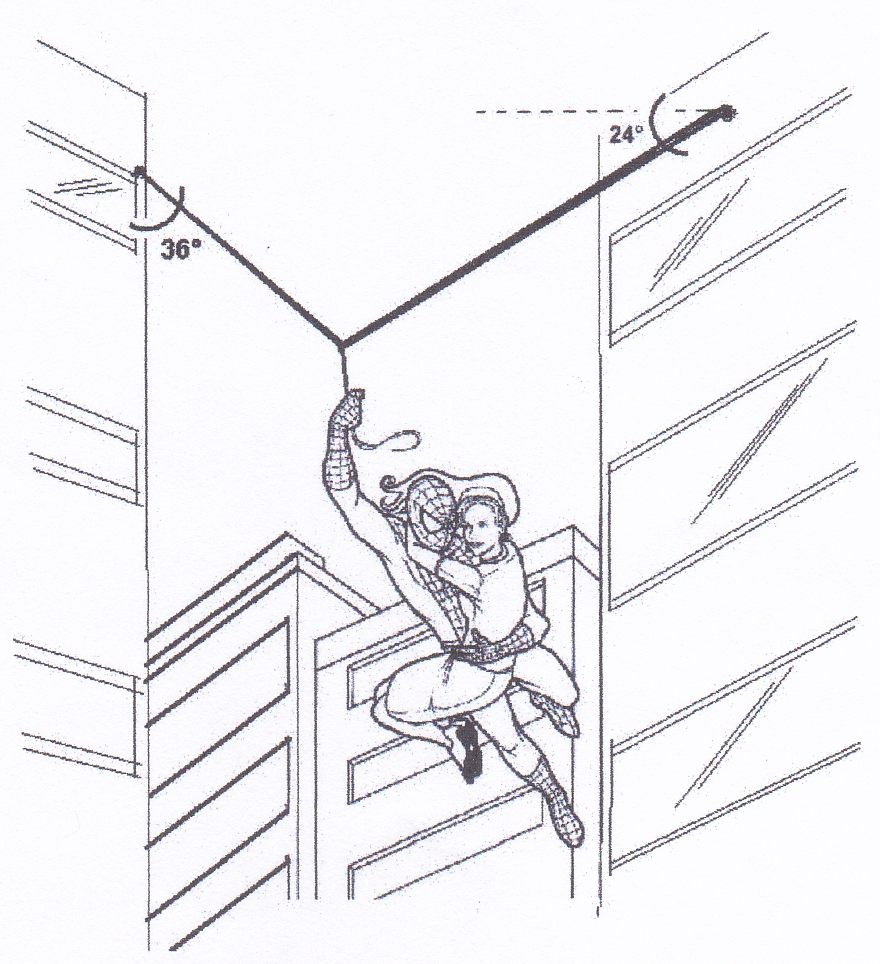
\includegraphics[scale=0.81]{Imagenes/DCL_Problema_07.png}
\end{figure}
\begin{tikzpicture}[overlay]
    \node at (4.2, 6) [color=ao] {\small{$T_{1}$}};
    \node at (6, 6.3) [color=ao] {\small{$T_{2}$}};
\end{tikzpicture}
\end{frame}
\begin{frame}
\frametitle{Revisando el enunciado}
El enunciado nos menciona que la masa el hombre araña y de la mujer, en total es de \SI{132}{\kilo\gram}, por lo que la fuerza debida a la aceleración de la gravedad es:
\pause
\begin{eqnarray*}
\begin{aligned}
W &= - m \, g = \pause - \SI{132}{\kilogram} \cdot \SI{9.81}{\meter\per\square\second} = \\[0.5em] \pause
&= - \SI{1294.92}{\newton}
\end{aligned}
\end{eqnarray*}
\pause
Esta fuerza la representamos con un vector cuya dirección está en el eje $y$ negativo.
\end{frame}
\begin{frame}
\frametitle{Diagrama de cuerpo libre}
\begin{figure}
\centering
\begin{tikzpicture}[scale=0.7]

    \draw (-3, 0) -- (3, 0);
    \draw [-stealth, thick, color=ao] (0, 0) -- (0, -4.31) node [right, midway] {\small{$- W$}};
    
    \pause
    
    \draw [-stealth, thick, color=red] (0, 0) -- (-2.36, 3.26) node [right, midway] {\small{$T_{1}$}};
    \draw (-2.36, 3.26) -- (-1, 3.26);
    \draw (-2.36, 3.26) -- (-2.36, 1.5);
    \draw (-2.36, 2.7) arc(270:306:0.5);
    \node at (-2, 2.3) {\small{$\alpha$}};
    \node at (-4, 2.5) {\small{$\alpha = \ang{36}$}};

    \pause

    \draw [color=red] (-1.81, 3.26) arc (0:-54:0.5);
    \node at (-1.5, 2.8) [color=red] {\small{$\theta_{1}$}};

    \draw [color=red] (-0.5, 0) arc(180:126:0.5);
    \node at (-1, 0.4) [color=red] {\small{$\theta_{1}$}};
    
    \pause
    
    \node at (-4, 1.8) {\small{$\theta_{1} = \ang{54}$}};
    \node at (-4.5, 1.1) {\small{$\alpha + \theta_{1} = \ang{90}$}};

    \pause
    
    \node at (4.3, 1.8) {\small{$\theta_{2} = \ang{24}$}};
    \draw (2.91, 2.57) -- (1.5, 2.57);
    \draw (2.91, 2.57) -- (2.91, 1.5);
    \draw [color=red] (2.4, 2.57) arc (180:204:0.9);
    \node at (1.8, 2.2) [color=red] {\small{$\theta_{2}$}};
    \draw [-stealth, thick, color=red] (0, 0) -- (2.91, 2.57) node [below, pos=0.7] {\small{$T_{2}$}};
    \draw [color=red] (0.5, 0) arc(0:42:0.5);
    \node at (1.2, 0.4) [color=red] {\small{$\theta_{2}$}};
    \onslide<1->
\end{tikzpicture}
\end{figure}
\end{frame}
\begin{frame}
\frametitle{Enlistando los vectores}
\begin{table}
\centering
\begin{tabular}{c | c}
Vector & Ángulo \\ \hline
$-W$ & \ang{270} \\ \hline
$T_{1}$ & \ang{54} \\ \hline
$T_{2}$ & \ang{24} \\ \hline
\end{tabular}
\end{table}
\end{frame}
\begin{frame}
\frametitle{Calculando las componentes}
\begin{table}
\centering
\begin{tabular}{c | c | c }
Componente & Expresión & Sustitución \\ \hline
$W_{x}$ & $(\cos \ang{270})(W)$ & $(0)(W)$ \\ \hline
$W_{y}$ & $(\sin \ang{270})(W)$ & $(-1)(W)$ \\ \hline
$T_{1x}$ & $-(\cos \ang{54})(T_{1})$ & $-(0.587)(T_{1})$ \\ \hline
$T_{1y}$ & $(\sin \ang{54})(T_{1})$ & $(0.809)(T_{1})$ \\ \hline
\end{tabular}
\end{table}
\end{frame}
\begin{frame}
\frametitle{Calculando las componentes}
\begin{table}
\centering
\begin{tabular}{c | c | c }
Componente & Expresión & Sustitución \\ \hline
$T_{2x}$ & $(\cos \ang{24})(T_{2})$ & $(0.913)(T_{2})$ \\ \hline
$T_{2y}$ & $(\sin \ang{24})(T_{2})$ & $(0.406)(T_{2})$ \\ \hline
\end{tabular}
\end{table}
\end{frame}
\begin{frame}
\frametitle{Condiciones de equilibrio}
Sabemos que si el sistema está en equilibrio, la suma de las componentes de las fuerzas tanto en la dirección $x$, como en $y$ valen cero:
\pause
\begin{eqnarray*}
\begin{aligned}
\nsum F_{x} &= 0 \\[0.5em] \pause 
\nsum F_{y} &= 0
\end{aligned}
\end{eqnarray*}
\end{frame}
\begin{frame}
\frametitle{Condiciones de equilibrio}
Para la componente en $x$ tendremos entonces:
\pause
\begin{eqnarray*}
\begin{aligned}
\nsum F_{x} &= T_{1x} + T_{2x} + W_{x} = 0 \\[0.5em] \pause
\nsum F_{x} &= (0.587)(T_{1}) + (0.913)(T_{2}) = 0
\end{aligned}
\end{eqnarray*}
\end{frame}
\begin{frame}
\frametitle{Condiciones de equilibrio}
Ahora para la componente en $y$ se tiene:
\pause
\begin{eqnarray*}
\begin{aligned}
\nsum F_{y} &= T_{1y} + T_{2y} - W_{y} = 0 \\[0.5em] \pause
\nsum F_{y} &= (0.809)(T_{1}) + (0.406)(T_{2}) - \SI{1294.92}{\newton} = 0
\end{aligned}
\end{eqnarray*}
\end{frame}
\begin{frame}
\frametitle{Sistema de dos ecuaciones}
Con las expresiones anteriores se obtiene un sistema de dos ecuaciones simultáneas con dos incógnitas:
\pause
\begin{align*}
-0.587 \cdot T_{1} + 0.913 \cdot T_{2} &= 0 \\[0.5em]
0.809 \cdot T_{1} + 0.406 \cdot T_{2} - \SI{1294.92}{\newton} &= 0
\end{align*}
\pause
De donde podemos utilizar cualquier técnica para resolver este sistema simultáneo de dos ecuaciones.
\end{frame}
\begin{frame}
\frametitle{Resolviendo el sistema de ecuaciones}
Acomodando los términos del sistema, se tiene:
\pause
\begin{align}
-0.587 \cdot T_{1} + 0.913 \cdot T_{2} &= 0 \label{eq:ecuacion_04} \\[0.5em] 
0.809 \cdot T_{1} + 0.406 \cdot T_{2} &= \SI{1294.92}{\newton} \label{eq:ecuacion_05}
\end{align}
\end{frame}
\begin{frame}
\frametitle{Resolviendo el sistema de ecuaciones}
De la ecuación (\ref{eq:ecuacion_04}) despejamos el valor de $T_{2}$:
\pause
\begin{eqnarray*}
\begin{aligned}
-0.587 \cdot T_{1} + 0.913 \cdot T_{2} &= 0 \\[0.5em] \pause
0.913 \cdot T_{2} &= 0.587 \cdot T_{1} \\[0.5em] \pause
T_{2} &= \dfrac{0.587}{0.913} \cdot T_{1} = \pause 0.643 \cdot T_{1}
\end{aligned}
\end{eqnarray*}
\end{frame}
\begin{frame}
\frametitle{Resolviendo las tensiones}
El valor anterior de $T_{2}$ lo sustituimos en la ecuación (\ref{eq:ecuacion_05}), para obtener $T_{1}$:
\pause
\begin{eqnarray*}
\begin{aligned}
0.809 \cdot T_{1} + 0.406 \cdot (0.643 \, T_{1}) &= \SI{1294.92}{\newton} \\[0.5em] \pause
0.809 \cdot T_{1} + 0.261 \cdot T_{1} &= \SI{1294.92}{\newton} \\[0.5em] \pause
1.0706 \cdot T_{1} &= \SI{1294.92}{\newton}
\end{aligned}
\end{eqnarray*}
\begin{eqnarray*}
T_{1} &= \dfrac{\SI{1294.92}{\newton}}{1.0706} = \pause \SI{1209.52}{\newton}
\end{eqnarray*}
\end{frame}
\begin{frame}
\frametitle{Obteniendo el segundo término}
Una vez obtenido $T_{1}$ usamos este valor para calcular $T_{2}$, para ello ocupamos la ecuación (\ref{eq:ecuacion_04})
\pause
\begin{eqnarray*}
\begin{aligned}
-0.587 \cdot T_{1} + 0.913 \cdot T_{2} &= 0 \\[0.5em] \pause
-0.587 \cdot \SI{1209.52}{\newton} + 0.913 \cdot T_{2} &= 0 \\[0.5em] \pause
- \SI{710.83}{\newton} + 0.913 \cdot T_{2} &= 0 \\[0.5em]
\end{aligned}
\end{eqnarray*}
\end{frame}
\begin{frame}
\frametitle{Obteniendo el segundo término}
\begin{eqnarray*}
\begin{aligned}
0.913 \cdot T_{2} &= \SI{710.83}{\newton} \\[0.5em] \pause
T_{2} &= \dfrac{\SI{710.83}{\newton}}{0.913} \\[0.5em] \pause
T_{2} &= \SI{777.65}{\newton}
\end{aligned}
\end{eqnarray*}
\end{frame}
\begin{frame}
\frametitle{Solución al ejercicio}
Una vez obtenidos los valores de las tensiones en las cuerdas, hemos resuelto el ejercicio.
\begin{align*}
T_{1} &= \SI{1209.52}{\newton} \\[0.5em]
T_{2} &= \SI{777.65}{\newton}
\end{align*}
\end{frame}

\subsection{Ejercio 8 - Guía}

\begin{frame}
\frametitle{Enunciado del Ejercicio 8}
Un anuncio de \SI{200}{\newton} se cuelga de un techo como se muestra en la figura, de manera que las cuerdas que lo sostienen forman un ángulo de \ang{90}.
\\
\bigskip
\pause
¿Cuál es la tensión en cada segmnento de la cuerda?
\end{frame}
\begin{frame}
\frametitle{Figura del Ejercicio 8}
\begin{figure}
  \centering
  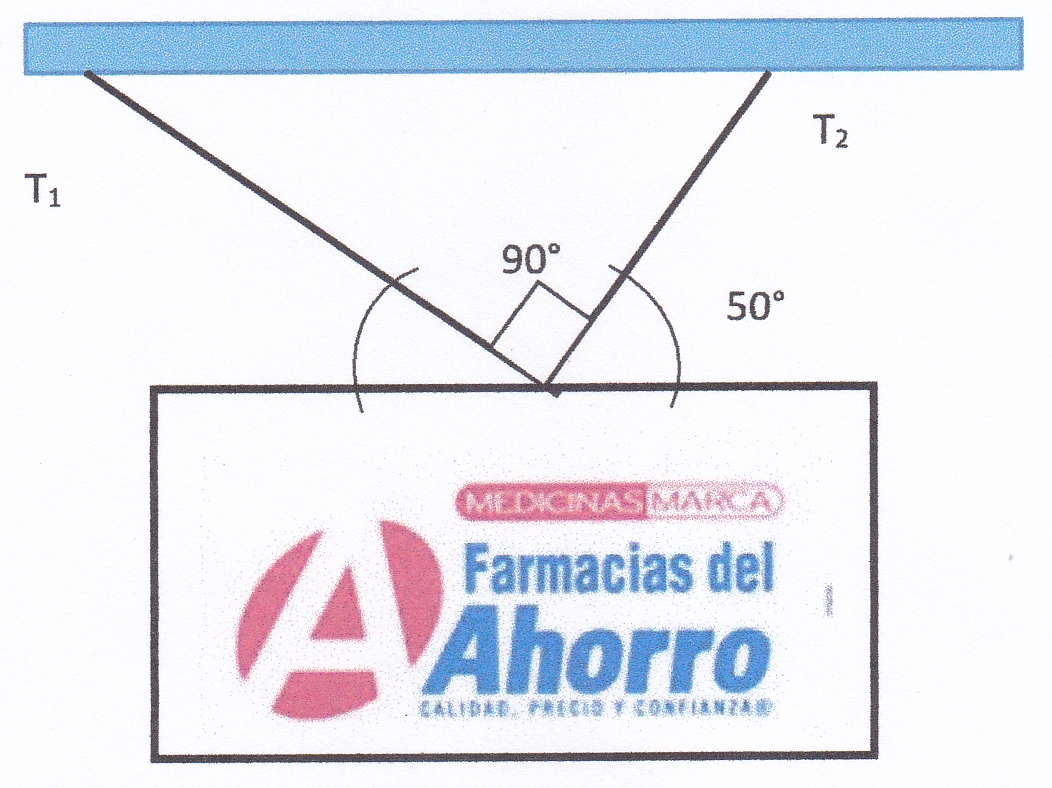
\includegraphics[scale=0.9]{Imagenes/DCL_Problema_08.png}
\end{figure}
\end{frame}

\end{document}